\documentclass[dvipdfmx,12pt]{beamer}
\usepackage{pxjahyper}
\usepackage{minijs}
\usepackage{amsmath}
\usepackage{fancybox}
\usepackage{array}
\usepackage{graphicx}
\usepackage{ascmac}
\usepackage{color}



\usetheme{Madrid}
\usecolortheme{default}
\renewcommand{\kanjifamilydefault}{\gtdefault}

\useoutertheme[subsection=false]{smoothbars}
\setbeamertemplate{footline}[page number]
\setbeamerfont{footline}{size=\small,series=\bfseries}
\setbeamercolor{footline}{fg=black,bg=black}

\newcommand{\backupbegin}{
  \newcounter{framenumberappendix}
  \setcounter{framenumberappendix}{\value{framenumber}}
}
\newcommand{\backupend}{
  \addtocounter{framenumberappendix}{-\value{framenumber}}
  \addtocounter{framenumber}{\value{framenumberappendix}} 
}





\title{最大の移動時間を最小化する教室割当問題の\\定式化と求解}
\author{\Large {システムモデリング研究室\\都11-0023 岡崎 俊介}}
\date{{\Large 2015年2月16日}}
\begin{document}

\begin{frame}\frametitle{}
\titlepage
\end{frame}

\begin{frame}\frametitle{先行研究での教室割当問題 \ (2013,鈴木)}
\begin{itemize}
\vspace{-5pt}
\item 教室割当とは\\
各授業をどの教室に割り当てるか
(現在手動で行われている)\\
\item 先行研究での教室割当問題の目標\\
\vspace{-3pt}
\begin{screen}
\begin{center}
\vspace{-3pt}
{\large  授業間の移動時間の総和が最小となる}\\
{\large  教室割当を求める}\\
\vspace{-5pt}
\end{center}
\end{screen}
\item 最適化問題として定式化・求解\\
\end{itemize}
\vspace{-7pt}
\hrulefill

先行研究の問題点\\
\begin{itemize}
\item 計算時間が長く,24通りのうち6通りしか解が求まらない\\
\item 目的関数が非常に複雑な構造になっている\\
\item 変数・制約数が多い\\
\end{itemize}
\end{frame}


\begin{frame}\frametitle{先行研究と本研究の目標の違い}
\begin{itemize}
\vspace{-3pt}
\item 先行研究での教室割当問題の目標(再掲)\\
\vspace{-3pt}
\begin{screen}
\begin{center}
\vspace{-3pt}
{\large  授業間の\textcolor{red}{移動時間の総和が最小}となる}\\
{\large  教室割当を求める}\\
\vspace{-5pt}
\end{center}
\end{screen}

\item 本研究での教室割当問題の目標\\
\begin{screen}
\begin{center}
\vspace{-2pt}
{\large 授業間の\textcolor{red}{最大の移動時間が最小}となる}\\
{\large 教室割当を求める}\\
\vspace{-3pt}
\end{center}
\end{screen}
\vspace{-5pt}
\begin{itemize}
\item 制約・変数の数が減る
\item 目的関数が分かりやすくなる
\end{itemize}
\end{itemize}
\end{frame}


\begin{frame}{定式化の例}
\begin{itemize}
\item 制約 \\
\begin{block}{各授業には必ず1つの教室を割り当てなければならない}
\vspace{-15pt}
\begin{eqnarray}
&&\sum_{i \in I} u_{i,j} = 1 \hspace{5.0mm}
\quad \left (\forall p \in P, \: \forall j \in JN_{p} \right)\nonumber
\end{eqnarray} 
\end{block}
$u_{i,j}$:授業$j$に教室$i$が割り当てられるとき,1となる変数
\vspace{10pt}
\item 目的関数\\
\begin{block}{制約の違反点数を最小化する}
\vspace{-15pt}
\begin{eqnarray}
\label{hmokuteki} 
&&\hspace{-70pt}{\rm minimize} \quad \sum_{pc \in PC} (pa_{pc} \cdot k_{pc}) \label{eqn:mokuteki}\nonumber
\end{eqnarray}
\end{block}
\end{itemize}
\end{frame}

\begin{frame}{数値実験の方法}
\begin{figure}[thpb]
\begin{center}
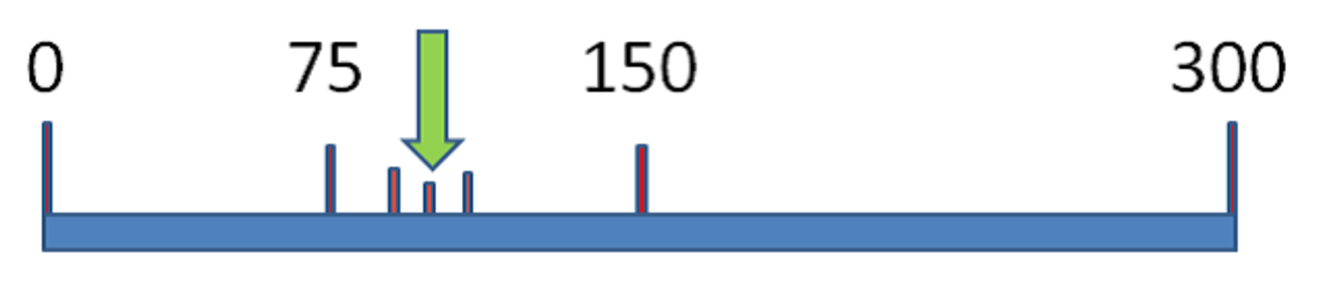
\includegraphics[scale=0.5]{nibuntansa.eps}
\hspace{-10mm} 
\vspace{-5mm}
\end{center}
\end{figure}

\begin{itemize}
\item 移動時間の上限を定めるパラメータ$r$を準備\\
\begin{screen}
\begin{center}
\vspace{-2mm}
実行可能解が得られるパラメータ$r$の最小値が\\最大移動時間の最小値
\vspace{-3mm}
\end{center}
\end{screen}
\item パラメータ$r$を調整しながら問題を解く\\
\item 実行可能解が得られるパラメータ$r$の最小値を求める\\
(目的関数の最小値が求めたい解ではない)
\item 全24通りの数値実験を行い,最大移動時間の最小値を求める\\

\end{itemize}
\end{frame}


\if0

\begin{frame}\frametitle{本実験}
\begin{itemize}
\item 本実験1:最大移動時間の最小値を求める実験\\
\vspace{5pt}
全24曜限(春・秋学期,月~土曜・午前・午後)で最小値を求める\\
\item 本実験2:本実験1の最小値が大きくなる授業を取り除いた実験\\
\vspace{5pt}
春学期月曜午後,春学期木曜午後の最小値が251秒と,他の曜限より大きい\\
\item 本実験3:希望教室を設定した,春学期火曜午前での実験\\
\vspace{5pt}
3つの1限の授業に,それぞれ同じ2教室を希望教室として設定する\\
\end{itemize}
\end{frame}
\fi

\begin{frame}\frametitle{最大移動時間の最小値}
\begin{table}
\begin{center}
\vspace{-5pt}
\begin{tabular}{|r|cc|c|}
\hline
\multicolumn{1}{|c|}{曜限} &  最大(秒)  & 平均(秒) & 計算時間(秒)\\
\hline
春学期月曜午前  & 96  & 58.3 &  4.34\\  
午後            & 251 & 53.6 &  0.44\\
火曜午前        & 76  & 39.4 &  1.04\\
午後            & 141 & 53.8 &  0.65\\
水曜午前        & 58  & 28.4 &  2.25\\
午後            & 52  & 18.0 & 19.41\\
木曜午前        & 34  & 14.1 &  1.53\\
午後            & 251 & 37.3 &  0.17\\
金曜午前        & 103 & 47.5 &  0.89\\
午後            & 74  & 20.9 &  2.01\\
土曜午前        & 33  & 12.6 &  0.27\\
午後            & 27  & 7.3  &  1.40\\
\hline                                        	         
\end{tabular}
\end{center}
\end{table}


\end{frame}


\begin{frame}\frametitle{最大移動時間の最小値}
\begin{table}
\begin{center}
\vspace{-5pt}
\begin{tabular}{|r|cc|c|}
\hline
\multicolumn{1}{|c|}{曜限} &  最大(秒)  & 平均(秒) & 計算時間(秒)\\
\hline
春学期月曜午前  & 96  & 58.3 & 4.34\\  
\hline                                        	         
\end{tabular}
\end{center}
\end{table}

\begin{figure}[thpb]
\begin{center}
\includegraphics[bb=0 0 390 248,clip,scale=0.7]{oMo12_pawapohist.eps}
\hspace{-10mm} 
\vspace{-5mm}
\caption{移動時間ごとの学生数(春学期月曜午前)}
\label{omo12}
\end{center}
\end{figure}


\end{frame}

\begin{frame}\frametitle{本研究と先行研究の実験結果の比較}
\begin{itemize}

\item 全24通りで最適解が求まった
\item 全ての計算時間が100秒以内
\begin{itemize}
\item 最も早い計算時間:0.13秒
\item 最も遅い計算時間:80.62秒
\item 平均計算時間:10.42秒
\end{itemize}

\begin{table}[h]
\begin{center}
\caption{本研究と先行研究の比較(春学期月曜午前)}
\vspace{-5pt}
\begin{tabular}{r|cc}
\hline
&本研究&先行研究 \\
\hline
移動時間(秒)& 96  & 最適解求解不可  \\  
制約数& 2569 &  933306 \\ 
変数の数&1854 & 4781 \\
計算時間(秒) &4.34&  3600.00\\
\hline
\end{tabular}
\end{center}
\end{table}
\item 制約数が大幅に小さくなっている
\item 変数の数はおよそ半数になっている
\end{itemize}
\end{frame}

\begin{frame}\frametitle{希望教室を設定した場合(春学期火曜午前)}
春学期火曜1限の3つの授業に希望教室を設定
\begin{table}[H]
\begin{center}
\begin{tabular}{|r|cc|c|}
\hline
 & 最大(秒) & 平均(秒) & 計算時間(秒)\\
\hline
希望教室なし  & 76  & 39.4 & 1.04\\
希望教室あり  & 76  & 47.9 & 1.73\\
\hline
\end{tabular}
\end{center}
\end{table}
\vspace{-4mm}

\begin{figure}[thpb]
\begin{center}
\includegraphics[bb=0 0 390 248,clip,scale=0.65]{otukarepawapo.eps}
\vspace{-3mm}
\caption{本実験1,3の移動時間ごとの学生数の比較}
\label{omo12}
\end{center}
\end{figure}

\end{frame}



\begin{frame}{まとめと今後の課題}
【まとめ】
\begin{itemize}
\item 先行研究とは異なる視点から教室割当問題を定式化・求解
\item 最大の移動時間を最小化する教室割当を,短い計算時間で求めることができた
\item 希望を考慮する教室割当も行える
\end{itemize}
【今後の課題】
\begin{itemize}
\item 最大でない移動時間の最小化
\item インターフェイスの開発
\end{itemize}

\end{frame}
\appendix
\backupbegin

\begin{frame}\frametitle{最大移動時間の最小値を求める実験}
\begin{table}
\begin{center}
\vspace{-5pt}
\begin{tabular}{|r|cc|c|}
\hline
\multicolumn{1}{|c|}{曜限} &  最大(秒)  & 平均(秒) & 計算時間(秒)\\
\hline
秋学期月曜午前  & 50  & 22.4 & 80.62\\
午後            & 67  & 27.3 &  3.29\\          
火曜午前        & 68  & 32.9 &  1.42\\
午後            & 49  & 12.5 & 42.46\\          
水曜午前        & 57  & 30.2 &  2.12\\
午後            & 123 & 43.1 &  0.56\\          
木曜午前        & 58  & 39.4 & 20.69\\
午後            & 60  & 21.7 & 60.58\\          
金曜午前        & 89  & 45.9 &  0.56\\
午後            & 80  & 28.4 &  2.96\\          
土曜午前        & 34  & 19.7 &  0.30\\
午後            & 74  & 52.7 &  0.13\\
\hline                                        	         
\end{tabular}
\end{center}
\end{table}


\end{frame}


\begin{frame}\frametitle{先行研究での制約条件・目的関数}
\begin{itemize}
\item 絶対制約(必ず守らなければならない制約)
\begin{itemize}
\item 1つの曜限における各教室には授業を1つしか割り当てられない
\item 各授業には必ず1つの教室を割り当てなければならない
\item 受講人数が教室の定員を超える授業を教室に割り当てられない
\item 特定の授業は指定された教室で開講されなければならない
\end{itemize}


\item 考慮制約(できるだけ守りたい制約)

\begin{itemize}
\item 特別連続授業は同じ教室で開講されることが好ましい
\item 移動時間は指定した時間以内であることが好ましい
\item 教室内の人が入れ替わる際の混雑が発生しないほうが好ましい
\end{itemize}
\item 目的関数\\
移動を行う全学生の移動時間の総和と,考慮制約を満たせて\\いない場合に発生する違反点数の合計を最小化
\end{itemize}
\end{frame}


\begin{frame}\frametitle{本研究での制約条件}
\begin{itemize}
\item 絶対制約(必ず守らなければならない制約)
\begin{itemize}
\item 1つの曜限における各教室には授業を1つしか割り当てられない
\item 各授業には必ず1つの教室を割り当てなければならない
\item 受講人数が教室の定員を超える授業を教室に割り当てられない
\item 特定の授業は指定された教室で開講されなければならない
\item 一般授業は特殊教室で開講されてはいけない
\item 特別連続授業は同じ教室で開講されることが好ましい
\item 移動時間は指定した時間以内であることが好ましい
\end{itemize}


\item 考慮制約(できるだけ守りたい制約)

\begin{itemize}
\item 教室内の人が入れ替わる際の混雑が発生しないほうが好ましい
\item 希望教室があれば,その教室で授業を開講したい
\end{itemize}
\end{itemize}
\end{frame}




\begin{frame}\frametitle{本実験2:特定の授業を取り除いた実験}
\begin{itemize}
\item 春学期月曜午後・春学期木曜午後で求まった最小値:\\他の曜限よりも大きい
\vspace{-10pt}

\begin{table}[H]
\caption{本実験1の結果}
\vspace{-5pt}
\begin{center}
\begin{tabular}{|r|ccc|}
\hline
 \multicolumn{1}{|c|}{曜限} &  最大(秒)  & 平均(秒) & 計算時間(秒)\\
\hline
春学期月曜午後  & 251 & 53.6 &  0.44\\
木曜午後        & 251 & 37.3 &  0.17\\
\hline
\end{tabular}
\end{center}
\end{table}

\item 平均移動時間と最大移動時間に大きな差がある
\item 特定の授業への移動時間が大きい
\item 移動時間の大きい授業を取り除いて再度計算を行ってみた
\end{itemize}

\end{frame}

\begin{frame}\frametitle{本実験2:特定の授業を取り除いた実験}
\begin{table}[H]
\caption{本実験2の結果}
\vspace{-5.0pt}
\begin{center}
\begin{tabular}{|r|ccc|}
\hline
\multicolumn{1}{|c|}{曜限} & 最大(秒) & 平均(秒) & 計算時間(秒)\\
\hline
春学期月曜午後  & 68 & 37.9 & 13.54\\
      木曜午後  & 51 & 15.4 & 1.84\\
\hline
\end{tabular}
\end{center}
\end{table}
\begin{itemize}
\item 最大移動時間を大幅に小さくすることができた
\item 平均移動時間も小さくなっている
\item 移動時間が大きくなりそうな授業の教室割当をあらかじめ決めておくことで,残りの授業に対するより良い教室割当を得た

\end{itemize}
\end{frame}

\begin{frame}\frametitle{本実験1,2の移動時間ごとの学生数の比較}

\begin{figure}[thpb]
\begin{center}
\vspace{-10mm}
\hspace{-11mm}
\includegraphics[bb=0 0 390 248,clip,scale=0.7,width=13cm]{omonagapawapo.eps}
\vspace{-3mm}
\caption{本実験1と本実験2の移動時間ごとの学生数の比較(春学期月曜午後)}
\label{omo12}
\end{center}

\end{figure}

\end{frame}



\begin{frame}\frametitle{本実験3:希望教室を設定した実験}
\begin{itemize}

\item 授業$j$に対する希望教室がある \\
研究室と近いetc...\\
\item 絶対制約にすると\\
希望が重なるかもしれないので向いていない\\
\item 考慮制約にする
\item 各授業を希望した教室で開講できない場合,目的関数に違反点数を加算

\end{itemize}
\begin{itemize}
\item 考慮制約に,希望教室を設けている
\item 本実験1では設定していない
\item 最大移動時間の最小値は変化するのか
\item 平均移動時間は変化するのか
\end{itemize}
\end{frame}


\begin{frame}\frametitle{改良点1}
\begin{itembox}[l]{考慮制約1 \ (先行研究)}
特別連続授業は同じ教室で開講されることが好ましい
\vspace{-10pt}
\[u_{i_1,j_1} + u_{i_2,j_2} -1\le \alpha_{j_1,j_2} 
\quad ((j_1,j_2) \in L ,i_1 \neq i_2)\]

\end{itembox}
\vspace{-15pt}
\[
u_{i,j} = \left\{
\begin{array}{ll}
1,& \text{教室$i$で授業$j$が開講されるとき} \hspace{30pt}\alpha\text{ :違反の指標}\\
0, & \text{それ以外} \hspace{120pt} L \text{:特別連続授業の集合 }
\end{array}
\right.
\]
 

\begin{itemize}
\item 特別連続授業(関連性の高い連続で開講される2つの授業):\\ほとんどの学生が連続受講\\
\item 教室移動すると混雑の可能性大\\
\item \textcolor{blue}{絶対制約にすることで混雑発生の可能性がなくなる}\\
\end{itemize}
\begin{block}{特別連続授業は同じ教室で開講しなければならない}
\vspace{-5pt}
\[ u_{i,j_1} = u_{i,j_2} \qquad ((j_1,j_2) \in L) \]
\end{block}

\end{frame}



\begin{frame}\frametitle{改良点2}
\vspace{-6pt}
\begin{itembox}[l]{考慮制約2 \ (先行研究)}
\vspace{-5pt}
 移動時間は指定した時間以内であることが好ましい\\
\vspace{-15pt}
\[w_{p,i_1,i_2}\cdot g_{i_1,i_2} \leq \beta_{j_1,j_2}\] \\
\vspace{-0.5in}
\end{itembox}
\begin{itemize}
\vspace{-5pt}
\item 制約式が正しくない\\

\item 休み時間は必ず一定時間以上ほしい\\
絶対制約にすることで確保する
\begin{block}{移動時間は指定した時間以内でなければならない}
教室$i_1$,$i_2$間で移動する学生の移動時間が指定した時間を越える場合,
\vspace{-10pt}
\[ u_{i_1,j_1}+u_{i_2,j_2}\le 1\]\\

\end{block}
\end{itemize}
\end{frame}




\begin{frame}\frametitle{改良点3-1}
\begin{itembox}[l]{考慮制約3 \ (先行研究)}
教室内の人が入れ替わる際の混雑が発生しないほうが好ましい\\
\vspace{-15pt}
\end{itembox}
\vspace{-15pt}
\begin{itemize}
\item 先行研究 :遠くの教室から来る人は混雑の対象とならない\\
\item 本研究:教室を出入りするすべての人が混雑の対象\\
(遠くの教室が早く授業終了,対象教室の授業終了が遅れるなど)\\
\begin{figure}

		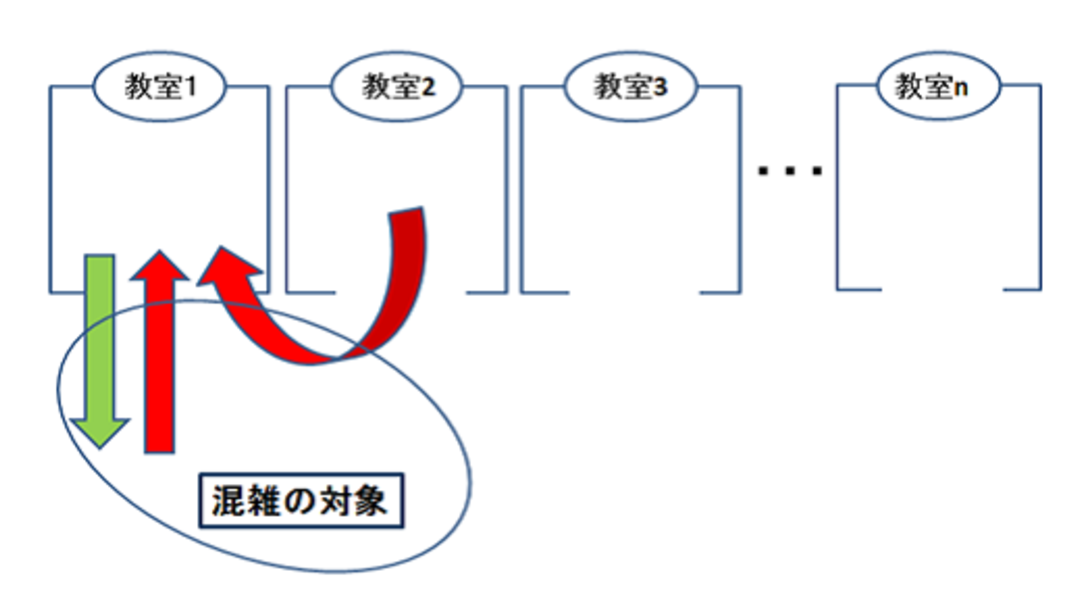
\includegraphics[width=7cm]{kouryo3_old8.eps}
	
\end{figure}
\end{itemize}
\end{frame}

\begin{frame}\frametitle{改良点3-2}
\begin{itembox}[l]{考慮制約3 \ (先行研究)}
教室内の人が入れ替わる際の混雑が発生しないほうが好ましい\\
\vspace{-15pt}
\end{itembox}
\vspace{-15pt}
\begin{itemize}
\item 先行研究 :遠くの教室から来る人は混雑の対象とならない\\
\item \textcolor{blue}{本研究:教室を出入りするすべての人が混雑の対象}\\
(遠くの教室が早く授業終了,対象教室の授業終了が遅れるなど)\\

\begin{figure}

		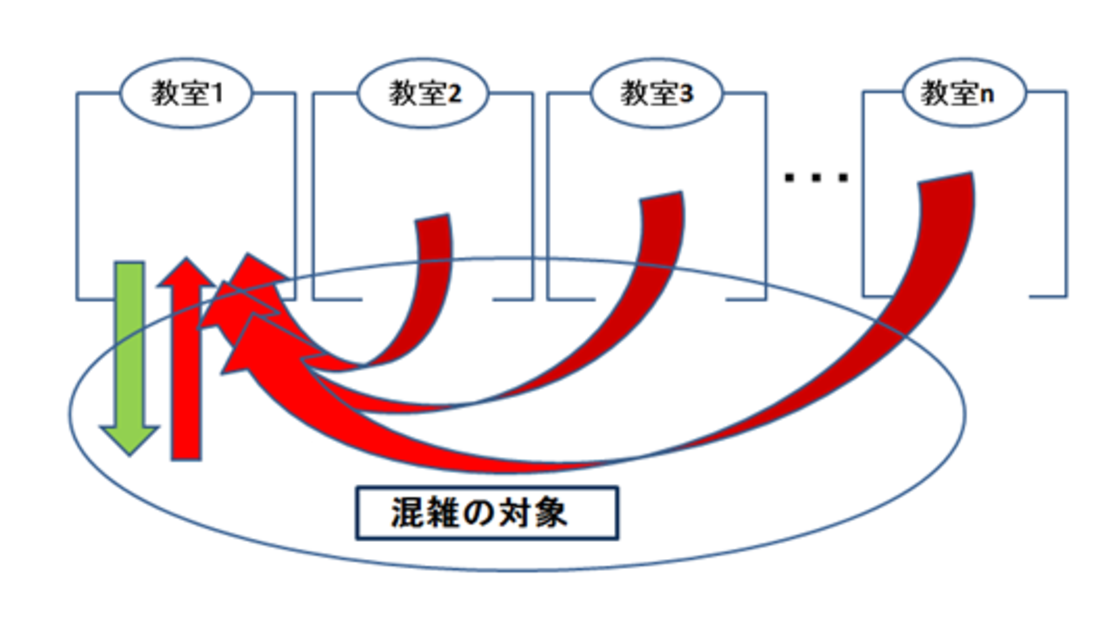
\includegraphics[width=7cm]{kouryo3_new8.eps}
	
\end{figure}
\end{itemize}
\end{frame}


\begin{frame}\frametitle{追加する制約条件}
\begin{itemize}

\item 授業$j$に対する希望教室がある \\
研究室と近いetc...\\
\item 絶対制約にすると\\
希望が重なるかもしれないので向いていない\\
\item 考慮制約にする

\begin{block}{授業$j$を希望教室で開講したい}
\[\text{違反点数} = \gamma \sum_j\sum_{i \in I \setminus I_j}u_{i,j} \]
\qquad \qquad ($I$:全教室の集合,$I_j$:授業$j$の希望教室の集合)
\end{block}
各授業を希望した教室で開講できない場合,目的関数に違反点数を加算

\end{itemize}
\end{frame}




\backupend
\end{document}
